%; whizzy chapter
% -initex iniptex -latex platex -format platex -bibtex jbibtex -fmt fmt
% 以上 whizzytex を使用する場合の設定。

%     Tokyo Debian Meeting resources
%     Copyright (C) 2007 Junichi Uekawa
%     Copyright (C) 2007 Nobuhiro Iwamatsu

%     This program is free software; you can redistribute it and/or modify
%     it under the terms of the GNU General Public License as published by
%     the Free Software Foundation; either version 2 of the License, or
%     (at your option) any later version.

%     This program is distributed in the hope that it will be useful,
%     but WITHOUT ANY WARRANTY; without even the implied warranty of
%     MERCHANTABILITY or FITNESS FOR A PARTICULAR PURPOSE.  See the
%     GNU General Public License for more details.

%     You should have received a copy of the GNU General Public License
%     along with this program; if not, write to the Free Software
%     Foundation, Inc., 51 Franklin St, Fifth Floor, Boston, MA  02110-1301 USA

%  preview (shell-command (concat "evince " (replace-regexp-in-string "tex$" "pdf"(buffer-file-name)) "&"))
% 画像ファイルを処理するためにはebbを利用してboundingboxを作成。
%(shell-command "cd image200701; ebb *.png")

%%ここからヘッダ開始。
\documentclass[mingoth,a4paper]{jsarticle}
\usepackage{monthlyreport}

% 日付を定義する、毎月変わります。
\newcommand{\debmtgyear}{2007}
\newcommand{\debmtgdate}{16}
\newcommand{\debmtgmonth}{6}
\newcommand{\debmtgnumber}{29}


% section の代わりの環境
\newcommand{\debconfsection}[2]{%
\newpage
第\debmtgnumber{}回 東京エリアDebian勉強会 \debmtgyear{}年\debmtgmonth{}月
%
% top line
\vspace{0.1mm}\\
\colorbox{dancerlightblue}{\hspace{\hsize}}
%
% middle text
%
\begin{minipage}[t]{0.7\hsize}
\color{dancerdarkblue}
\vspace{1cm}
\section{#1}
\hfill{}#2\\
\end{minipage}
\begin{minipage}[t]{0.3\hsize}
\vspace{-2cm}
\hfill{}
\includegraphics[height=5cm]{image200706/logo-banner-split1.png}\\
\vspace{-5cm}
\end{minipage}
%
%
%vspace{-2cm}\\
\colorbox{dancerdarkblue}{\hspace{\hsize}}
%
\vspace{2cm}
}

\begin{document}

\begin{titlepage}

% 毎月変更する部分, 本文の末尾も修正することをわすれずに


 第\debmtgnumber{}回 東京エリア Debian 勉強会資料

\vspace{2cm}

\begin{minipage}[t]{0.6\hsize}
\vspace{-2cm}
{\fontsize{60}{60}
{\gt
東京エリア \\
デビアン \\
勉強会
}}
\end{minipage}
\begin{minipage}[b]{0.4\hsize}
\hspace{-1cm}
\includegraphics[width=9cm]{image200502/openlogo-nd.eps}
\end{minipage}

\vspace{3cm}
\hfill{}Debian勉強会幹事 上川 純一\\
\hfill{}\debmtgyear{}年\debmtgmonth{}月\debmtgdate{}日

\thispagestyle{empty}
\end{titlepage}

\dancersection{Introduction}{上川 純一}
 
 今月のDebian勉強会へようこそ。
 これからDebianのあやしい世界に入るという方も、すでにどっぷりとつかってい
 るという方も、月に一回Debianについて語りませんか?

 目的として次の二つを考えています。

 \begin{itemize}
 \item メールではよみとれない、もしくはよみとってられないような情報につ
       いて情報共有する場をつくる
 \item Debianを利用する際の情報をまとめて、ある程度の塊として整理するた
       めの場をつくる
 \end{itemize}

 Debianの勉強会ということで究極的には参加者全員がDebian Packageをがりがり
 と作るスーパーハッカーになった姿を妄想しています。

 Debianをこれからどうするという能動的な展開への土台としての空間を提供し、
 情報の共有をしたい、というのが目的です。


\newpage

\begin{minipage}[b]{0.2\hsize}
 \colorbox{dancerlightblue}{\rotatebox{90}{\fontsize{80}{80} {\gt デビアン勉強会} }}
\end{minipage}
\begin{minipage}[b]{0.8\hsize}
\hrule
\vspace{2mm}
\hrule
\tableofcontents
\vspace{2mm}
\hrule
\end{minipage}


\dancersection{最近のDebian関連のミーティング報告}{上川 純一}

\subsection{東京エリアDebian勉強会28回目報告}
% (query-replace-regexp "<.*?>" "")
% (query-replace-regexp "^[ 	]*" "")

東京エリアDebian勉強会参加報告。
5月の第28回東京エリアDebian勉強会を実施しました。

今回の参加者は
前田さん、やまねさん、出井さん、kinnekoさん、
hamanoさん、小室さん、鈴木さん、武藤さん、
山下さん、あけどさん、岩松さん、
noriaki satoさん、山本浩之さん、
山辺義孝さん、本庄さん、キタハラさん、
鈴木邦男さん、えとーさん、荒木さん、David Smith さん、
Charles Plessy さん、後藤さん、上川の23 人でした。

最近のイベントの紹介として、最初に前回の報告を行いました。
前回は主要な分散バージョン管理ツールについての特集でした。

DWNクイズを今回も実施しました。
全員に起立してもらい、グー・チョキ・パーで選択してもらいました。
1問目は一人しか正解しませんでした。
alioth にて、 git は昔からサポートされていており、今回サポートが追加されたのはMercurialです。
しかたないので、2問目からしきりなおし、最後まで4人ほどのこりました。
勝者には上川からここには書けないような豪華景品を贈呈しました。おめでとうございます。


次に、Debian Conferenceに向けて実施している準備の紹介を行いました。
pbuilder と superh についてのプレゼンテーションを行うことになっているの
ですが、リハーサルとして、Debian勉強会にて今回内容を説明しました。

最初にpbuilder について上川が紹介しました。
Debian ソースパッケージを処理してバイナリをつくる際に、
クリーンルーム環境を利用する、その手順をまとめたツールです、ということを紹介しました。


次に岩松さんが Debian の superh の移植版の紹介をしていました。
過去の歴史について力をいれて紹介していました。

kinneko さんがSH2A版のポートをやっている人もいるので紹介するのがよいだろうという指摘をしました。

上川の感想ですが、Debconfで紹介する目的として、新しい開発
者を募集するのが目的なのであれば、歴史については簡単にまと
めてしまって、SuperHの開発に使える機種の情報や何が面白いの
か、現状のポートのステータス、連絡先やレポジトリやウェブサ
イトの情報、どういう課題があるのかに力をいれて紹介するのが
よいのではないかという印象をうけました。

小室さんがその後に「サーバをエッチにしてみました」という題
でネタを披露しました。いろいろとトラブルがありそれを解決し
ました、ということだったのですが、「エッチにアップグレード
するのは簡単だということがわかりました」というので話をしめ
たので一同爆笑しました。


いつもとタイミングを変えてみて、その後に事前課題の紹介を行
いました。内容は「エッチになって困った事」にしてみました。
みんないろいろと思うところがあるようで議論が沸騰しました。
webminがなくなったこと、xlock がないこと、xorg になってし
まい設定が大きく変わっていること、udev の使いかたがよくわ
からないこと、カーネルがアップグレードするのでカーネル関連
の問題(ACPIなど)にぶつかる可能性があること、などが話題に
でました。/var/lock/apache2/ の権限が www-data ではなく 
root になってしまっているので webdav で書き込めないことな
どが紹介されていました(\debianbug{420101})。
apt-setup が削除されているのも仕様ですね。CUIで sources.list を編集するツールがあるのか?という話題が出ましたが、 vi をつかえ、と。

エッチにアップグレードする際に、どうやってみんなは情報をえ
ていて、どういうふうに情報を提供しているのだろう、という話
をしました。リリースノートを読むだとか、バグレポートを探す
だとか、MLに投稿するだとか、建前はおいておいて、現実のフロー
がどうなっているのかを語ってみました。どうやら、問題があれ
ばIRCでまず質問してみて、google で検索してみて、いろいろと
ためした結果を blog に書いている、というのが現実的なようで
す。そして、2ch などで同様の質問がされたら、 blogで書かれ
ている内容をまとめなおしてスレッドテンプレにまとめなおされ
るという流れになっているようです。言語が英語である点などか
らBTSは敷居の高く感じている人が多いようで、また複合的な問
題はパッケージ単位でしか登録できないBTSにはそぐわないため、
そういう情報の流れになっているようです。現実を見据えて今後
どうしていくべきか、悩ましいところです。

今回は宴会は
時の居酒屋  刻 荻窪店
にて開催しました。
料理がおいしかったです。

\debconfsection{Debconf 2007 各種討議内容}{岩松 信洋、矢吹 幸治、上川 純一}
\label{sec:debconf2007detail}
\index{Debconf2007}
\index{Debconf}

2007年度の Debconf は 6月13日から6月23日まで、スコットランド、エジンバ
ラで開催されました。2007年度の Debconf の討議内容を以下にまとめます。


\subsection{6月16日の発表内容}
\subsubsection{simple-CDD}

CDD を簡単に準備できる仕組み。reprepro を使ってミラーを作成している。
debpartial などはうまくうごかないことが多かったらしい。会場からはなぜ
aptitude とかを利用しないのかという質問は出ましたが、そこまで検討してい
ない、とのことでした。

\texttt{--qemu} オプションを指定したらイメージを作成して qemu でテストす
るところまでしてくれるそうです。\texttt{build-simple-cdd} コマンドを使えば簡単に
CDDがつくれるそうです。

\subsubsection{64studio}
Debian ベースの音楽関係のソフトウェアを収録したCDD(Common Debian
Distribution)です。各音源を組み合わせて、音を組み上げていくJackというプ
ログラムの説明などをしていました。イコライザーとしてJaminを利用し、出力
の周波数特性をフリーハンドで変えることができるデモをしていました。また、
PCのキーボードをつかって、パイプオルガンシミュレータ aeolus の(鍵盤の)キー
ボードを使って演奏するデモもしていました。

\subsection{6月17日の発表内容}
\subsubsection{Welcome talk}
  開会の挨拶。スポンサーと開催にかかわってくれた人たちへの感謝のコメントを
  行いました。非常にシンプルに終わった開会式でした。
	
\subsubsection{About porting SuperH for Debian}
  Renesas 社製 CPU SuperH の Debian へのポーティングの話でした。SuperH を 
  Debian にポーティングしている途中経過と現在発生している問題、および今後
  の課題について話し合いました。組込み関係の人が参加してくれていたが、みな 
  ARM にかかわっているので直接の支援は難しそうな印象をうけました。

\subsection{6月18日の発表内容}

\subsubsection{bugs.debian.org and debbugs}

BTS の開発についての進捗報告でした。いろいろな機能が追加されているのです
が、歴史的経緯でdone状態の遷移とバージョントラッキングで問題が解決してい
るかどうかという状態の遷移に整合性がとれないようになっているという話題が
でました。この部分については互換性をなくしてでも解決してよいのではないか、
という討論をしました。また、SOAPインタフェースの新しい機能の紹介などもあ
りました。

\subsubsection{Embedded Debian}

  Debian の組込み向けプロジェクト Emdebian の話です。今まで行ってきた方
  法の説明と結果を報告し、今後の方向性について話しをしました。 現在の 
  ftp-master 達はクロスビルドは受け付けてくれません。この問題を解決する
  ためにパッケージにタグを付けたりして対策する予定とのことです。
  Embedded 用のツールも用意しており、これらを使ってクロスビルドできるよ
  うになりました。 しかし、全てのパッケージはチェックできず
  \begin{commandline}
  make check
  \end{commandline}
  や
  \begin{commandline}
  make nodocs
  make nocheck
  \end{commandline}
  を使うように修正する必要があることを提案しました。
  その他の問題は後日行われた BOF で議論されました。

\subsubsection{Debian Live}
 Debianのサブプロジェクトとして活動しています。ツールは Ubuntu の casper 
 からforkして作成したものです。国際化も国コードやキーボードを入れるよう
 にするみたいです。自分で会社を興して、キオスクシステムのために開発をし
 たとのこと。また、usb ブートなどもサポートしているので、コンピュータ本
 体に情報が残らなく、銀行などからも引合があると話していた。こちらから
 i18nに関連した質問をしたら、日本の市場に興味があるようで、あとで、すで
 に作ってあった日本用のCD イメージを見せてくれました。

 \url{http://download.webconverger.com/i18n/jp/webc-2.21.jp.iso} からダウンロー
 ドできます。

\subsubsection{Debian Armel Port}

Armel の Debian へのポーティングの話でした。

\subsubsection{OpenStreetMap}
  Free な地図をつくるためのプロジェクトの話です。Google Map がすでに存在し
  ていますが、DFSG-Free ではないので、GPS 等を使って、自由に扱える地図を
  つくるということが目的です。ライセンスは Creative Commons を採用しています。

  \url{http://www.openstreetmap.org}

\subsubsection{Wacky Ideas II}
  Wacky Ideas というのは、こんな凄いこと考え付いちゃったぜというのを、ディ
  スカッションしてまともなものにしていく、ブレーンストーミング系のセッショ
  ンです。

  口火をきったのは、 Ian Jackson による upstream, ディストリビューション, 
  派生ディストリビューションで無駄なことしてないか? これらを包括するよう
  なVCS(Version Control System)って作れないか? って話。

  次は、Ubuntu の言語パックのように、翻訳 debを作るべきかと言う話題でし
  た。この方法は翻訳の部分が小さいのであればオーバヘッドが大きすぎる。そ
  のためパッケージをまとめて扱うことになるだろうとうことでした。極端なや
  り方として Ubuntu は、(1つで) 100MB のパッケージとして対処しているとい
  うことです。

\subsection{6月19日の発表内容}
\subsubsection{Debian virtualization support}
  Debian での仮想化ツールサポートの話です。あらゆる仮想化のシステムをサポートし、
  それらをサポートするための独自のツールを開発していることを紹介しました。
  また、仮想化ツールを使った、Debian パッケージのメンテナンスの話をし、
  ユーザー側だけでなく、開発者側から使い易くするために行っている活動をアピール
  していました。

\subsubsection{From Concept to Concrete}
  ハードウェアの企画、提案、そしてできるまでを、 Daniel Silverstone と 
  Vincent Sanders がコント風で行っていました。自分たちのハードウェア設計
  会社の紹介をしたかっただけなのかもしれないです。

\subsubsection{PC Install and Backup Management}
  発表者が来れなかったので、集まったみんなでディスカッションして進めるこ
  とになりました。まず、みんなどんなツールを使っているかと言う話題になり
  ました。

  unstableに、boxbackupというソフトウェアがあるから使っているいう人から、
  mondo, rsync, cpio, tar などを使っている人もいました。また、サーバ上でシステ
  ムをバックアップするために lvm-snapshot を使わないといけないんだという人
  は、Mysqlのデータベースの同期機能を利用していました。

  つぎに話題は、d-i (Debian Installer) を使って、大量にインストールする話
  題になりました。preeditを使って同じようにインストールする手法や、FAIを使う方
  法などがでてきました。


\subsubsection{Debconf 9 Presentations}
  Debconf 9 のプレゼンテーションです。
  Debconf 8 は アルゼンチンに決定しているが、
  Debconf 9 はまだ未定です。このセッションでは、Debconf 9 の立候補地域による
  プレゼンテーションを行いました。
  現在のところ、立候補地はスペインの Extremadura のみです。
  食事施設や宿泊施設が充実しており、プールもあるとのことです。
  この流れだと Debconf9 は Extremadura に決まりそうです。
  詳細は \url{http://wiki.debconf.org/wiki/Extremadura} からみることができます。

\subsubsection{Emdebian BOF}

  Debian の組込向けプロジェクトである Emdebian の BOF でした。uClibc の
  サポートおよび、busybox をベースにしたユーザーランドのサポートについて
  議論しました。既にサポートの体制を整えるようにしているが、uClibc をサ
  ポートしてしまうと、uClibc 用のバイナリを作成する必要があるので、バイ
  ナリの数が倍になってしまいます。この問題をどのように解決していくか、今
  後議論を重ねていくとのことです。

  Busybox の話は、busybox をベースにした場合、動くパッケージと動かないパッケージが
  出てしまいます。これは busybox をベースとして使用しているため発生する問題です。
  組込みでは busybox の base system を考える必要があるので、現在どのパッケージが動かない
  のかを調査している段階です。調査した結果は wiki にまとめられています。
  \url{http://wiki.debian.org/EmdebianRootfs}

\subsubsection{Keysigning Party}

今年は、キーサインに集まった人達を4つのグループに分けて、各グループを大
きめの部屋で分割してキーサインを行いました。全員がキーサインをするには巨大な
場所が必要だったので分割したのでしょう。

キーサインには finterprint を印刷した紙が必要です。そこに計算したsha1の
結果を書き込んで持参するのですが、その値
(sha1sum出力)が読み上げられ、同じ結果が出たことが確認できた人だけが書名
できます。

各人は国家の発行する公的な写真つきの証明書(例えばパスポート)を見せ、
fingerprint, sha1の計算結果について確認していきます。

分割したおかげか今年は30分程度で終わりました。

\subsection{6月20日の発表内容}
\subsubsection{Daytrip}

Debconf では一日、参加者で旅行をするというイベントがあります。今回の
Debconfでは Rotheway (Bute島) でまったりとピクニックをしました。Rotheway 
への移動は、Edinburgh から Glasgow へ電車で移動し、Glasgow からさらに電
車で Wemyss Bay へ移動します。Wemyss Bay は Rotheway 行き専用の舟着き場
で、そこから船に乗って Rotheway に移動しました。

\begin{wrapfigure}{r}{5cm}
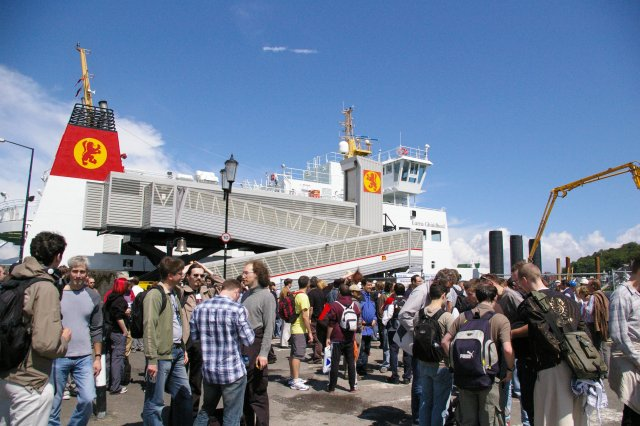
\includegraphics[width=5cm]{image200706/debconf7-daytrip.jpg}
\end{wrapfigure}

Rotheway の町は島で、特になにもないところです。ほとんどの建物は売出中で、
裁判所の建物も売りに出ていました。財政がやばそうな感じです。
建造物としては、教会や、バイキングの侵略の際に戦った城がありましたが、修復中でしかも工事は止まっていました。
山の奥へ1時間ほど歩くと、湖があり、大抵の参加者はその湖でピクニックをしたり、ボード
に乗って遊んでいたようです。

\subsection{6月21日の発表内容}
\subsubsection{Forking Debian every day}

GNU arch でいかに SELINUX版のDebianのポーティングを楽にしたか、というワー
クフロー紹介のセッションのはずでしたが、いろいろと技術的な障害があったよ
うで、 git でDebianのパッケージをメンテナンスするための方法をデモンスト
レーションするセッションに急遽変更されました。アプリケーションの各種機能
をSCMのブランチの機能を利用して実装し、新しいバージョンがリリースされて
もSCMの機能が活用できる、という話題でした。

\subsubsection{Quality assurance activities for localization}

小林さんが提案を提出し通っていたのですが、なぜか Debconf7 に参加しなかっ
たのと、報告・周知・対策を何も講じなかったため開催されるはめになりました。

急遽 IRC で現地と日本を結んで上川がセッションを行いました。フランス、ブ
ラジルなどのチームでの翻訳の進め方やツールの使い方についてディスカッショ
ンを行いました。メーリングリストをスキャンしてくれるロボットツールがあ
り、日本翻訳チーム向けに使えるように調整してくれるとのことでした。

\subsubsection{Debian ceilidh/Sun Drinks Reception}
\begin{wrapfigure}{r}{5cm}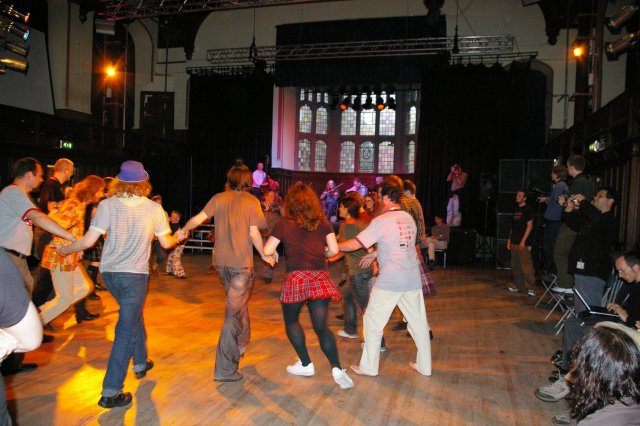
\includegraphics[width=5cm]{image200706/debconf7-dance.jpg}\end{wrapfigure}

Sun Microsystems と Google のスポンサによるパーティでした。Sun が飲み物、
Google がピザを提供してくれました。また、スコットランドの民謡の演奏家を呼
び、大ホールに集まったパーティ参加者達でスコットランドのダンスを楽しみま
した。

\subsection{6月22日の発表内容}

\subsubsection{Derivatives Round Tables --- Debianより派生したディストリビューション}

Benjamin ``Mako'' Hill が司会を務める、Debian より派生したディストリビュー
ションの関係者が集まってのパネルセッションでした。ベネズエラで開発されて
いる国の支援を受けたディストリビューション、スペインの Extremadura、
Debian Edu, Ubuntuなどが参加してきていました。予想どおり白熱しました。ディ
ストリビューションからのフィードバックの部分が問題になっていました。BTS 
の共有などもトピックになっていました。

\subsubsection{Proactive Bug Discovery}

  DPLである、Sam Hocevar のセッションでした。
\footnote{このセッションの英語は矢吹にはわかりやす
  かった。}ソースを全部チェックするのは非常にコストが高いので、クリティカ
  ルな部分だけは全部査読するが、ほとんどの部分は、ツールを使って機械的に
  チェックするだけもかなりのことがわかるとのことでした。

ソースコードを正規表現でスキャンしたり、google のコードサーチエンジンで
  チェックしたり、コンパイラーにチェックさせたりという部分について語って
  くれました。

\subsection{6月23日の発表内容}

\subsubsection{debian-community.org}

  Debianコミュニティに対する問題意識から、
  \url{http://debian-community.org} の提案セッションが行われました。
  Ubuntuコミュニティの事例からとったものです。Debian開発者になり活躍する
  までの時間がかかるのが問題意識となっています。その問題を解決するべく、
  debian-community.orgというサイトを作り、Debianコミュニティ活動すると宣
  言し、活動している間はメールの転送などのサービスを提供します。活動が一定
  期間止まったら、この活動リストより外されます。他にもplanetや、wikiなどの
  提供を行う予定があります。

  問題点としては、これまでのローカルコミュニティとの整合性、debian.org 本
  体もコミュニティであること、新しいコミュニティを作ってドライブしていく
  だけの魅力がそこにあるかなどが話し合われました。

\subsubsection{WTFM, again: Write The Fine Manual page}

Debian package で頒布されているプログラムには man が付属していないと
いけないということが Debian Policy で決まっているが、nroff 形式の man
は時代遅れです。man だけでなく、あらゆるフォーマットに対応したドキュメントを
容易に作成するにはどうしたいいのか話し、DocBook XML を使った場合の簡単な
チュートリアルを行いました。
また、man はあるが、Linux の man ではく、Unix の man だったりすることが
あるので、ユーザーに man を提供する際に注意すべき事などを話しました。

Debian package で頒布されているプログラムには man が付属していないといけ
ないということが Debian Policy で決まっているが、norff 形式の man は時代
遅れです。man だけでなく、あらゆるフォーマットに対応したドキュメントを容
易に作成するにはどうしたいいのか話し、DocBook XML を使った場合の簡単な
チュートリアルを行いました。また、man はあるが、Linux の man ではく、
Unix の man だったりすることがあるので、ユーザーに man を提供する際に書
いてある内容が本当に妥当なのか確認すべき事などを話しました。
 
\subsubsection{pbuilder talk}

上川 純一 がpbuilder, cowbuilder, qemubuilder についての議論を行いました。
pbuilder を利用しているユーザは非常に多いが、qemubuilder の利用者は数人
もいなかったということがわかりました。また、マニュアルの存在をしらない 
人が多数いました。

\subsubsection{Lightning Talks}

ライトニングトークは若干オーガナイズに失敗しており、最初計画していたメン
バーがあまりいなかったため、好きな人が好きなことを語るという会になってし
まいました。

\subsubsection{Closing ceremony}

最後のしめの挨拶がなされ、スポンサーに感謝したりしました。

\subsection{講演以外のできごと}

\subsubsection{apt-listbugs 関連の討論}

Don Armstrong がきており、bugs.debian.org の SOAPインタフェースを拡張し
た、といいました。apt-listbugs の実装を変更し、SOAPインタフェースを利用
するようにし、現在サーバ側で生成しているインデックスファイルが、もう必要
ないようにしました。現地で SOAP インタフェースのデバッグを実施し、実用に
なるようにしました。

また、 debian-changelog-mode に以前パッチをおくってくれた Luca Capello 
と BTS の HTML をパースしているからださいんだよ、という話をしたら、 SOAP 
を emacs からつかうのはいやなので、apt-listbugs を使おうという話になり、 
apt-listbugs list コマンドを拡張して実装することになりました。しかし、そ
れが実装されるまえに、vim のメンテナ Stefano Zacchioli がその話をうしろ
で聞いていて、その場でvim 用の debian/changelog での closes: 補完コードが
実装されてしまいました。

\subsubsection{QEMU 関連の討論}

上川は qemu、qemubuilder 関連であつく議論してまわりました。

Thiemo Seufer (QEMU mips ポートのメンテナで QEMU のコミッタ、および
Debian の MIPS ポートのメンテナ)と議論しました。chroot 内部での qemu
user emulation をいかに static link をしないで実施するのか、という点につ
いて議論し、環境変数を定義する必要があるね、ということで合意しました。

夕食の時間で Ottavio と議論し、qemubuilder の設計と、qemu system
emulation ではなく qemu user emulation での実装について議論しました。


\subsubsection{矢吹×grisu}

aptにi18n機能がマージされたのにまだサーバ側のインフラの整備が行われていま
せん。矢吹はDDTPの担当者の Grisu と DDTP の展開について議論しているようで
した。なんらかの成果がでるとよいですね。

\subsection{来年の Debconf}

来年の Debconf はアルゼンチンで8月に行われます。日本は夏ですが、アルゼン
チンは冬です。冬期合宿になると思いますので、気合いをいれていかないと、ひ
どいことになるかもしれません。気を付けましょう。

\cleartooddpage

\begin{minipage}[b]{0.2\hsize}
 \colorbox{dancerlightblue}{\rotatebox{90}{\fontsize{80}{80} {\gt デビアン勉強会} }}
\end{minipage}
\begin{minipage}[b]{0.8\hsize}

\vspace*{15cm}
\hrule
\vspace{2mm}

\includegraphics[width=2cm]{image200502/openlogo-nd.eps}
\noindent \Large \bf Debian 勉強会資料\\ \\
\noindent \normalfont \debmtgyear{}年\debmtgmonth{}月\debmtgdate{}日 \hspace{5mm}  初版第1刷発行\\
\noindent \normalfont 東京エリア Debian 勉強会 (編集・印刷・発行)\\
\hrule
\end{minipage}

\end{document}
